% Copyright (c) 2024, Francisco Fernandez
% License: CC BY-SA 4.0
%   https://github.com/fernandezfran/thesis/blob/main/LICENSE
\subsection{Orden de corto alcance}

El término orden de corto alcance (SRO, de sus siglas en inglés 
\textit{short-range order}) se utiliza para denotar el ordenamiento de los átomos
que rodean a uno específico en una cáscara determinada. Del mismo modo, el término 
\textit{clustering} se ha definido como la tendencia de los átomos similares a 
estar cerca unos de otros. Ambos conceptos se refieren a un orden estructural 
entre átomos vecinos, pero no son necesariamente persistentes a distancias más 
largas. Warren \cite{warren69} y Cowley \cite{cowley1950} definieron un 
parámetro (WCP) para caracterizar estos tipos de ordenamientos de la siguiente 
manera:
\begin{equation}
    \text{WCP} = 1 - \frac{p_{\text{A}-\text{B}}}{m_\text{B}} = 1 - \frac{p_{\text{B}-\text{A}}}{m_\text{A}},
\end{equation}
donde $p_{\text{A}-\text{B}}$ ($p_{\text{B}-\text{A}}$) es la probabilidad de tener un átomo de tipo B (A) como
vecino de un átomo de tipo A (B) y $m_\text{B}$ ($m_\text{A}$) es la concentración global de átomos
B (A), expresadas en fracciones molares. La igualdad, en ambas definiciones 
posibles del WCP, viene del hecho de que la probabilidad de encontrar a un átomo 
de tipo A como vecino de un átomo de tipo B es igual a la de tener un átomo de 
tipo B como vecino de un átomo de tipo A, esto es $m_\text{A} p_{\text{A}-\text{B}} = m_\text{B} p_{\text{B}-\text{A}}$.

Los valores que se obtienen de utilizar el parámetro WCP en sistemas del tipo
A$_x$B indica una aleatoriedad completa si es igual a cero, preferencia por 
átomos de distinto tipo si WCP$ < 0$ y preferencia por átomos del mismo tipo si 
WCP$ > 0$. Aunque este parámetro permite un análisis cuantitativo notable, sólo
se define para sistemas cristalinos en los que cada átomo tiene el mismo número
de vecinos \cite{warren69}.

A continuación se extiende esta idea para definir un nuevo parámetro, 
$\theta_{\text{A}-\text{B}}$, que es adecuado para caracterizar estructuras amorfas, de la 
siguiente manera:
\begin{equation}
    \theta_{\text{A}-\text{B}} = \ln \left( \frac{C_{\text{A}-\text{B}}}{C_{\text{Bulk}}} \right),
\end{equation}
donde A indica la naturaleza del átomo que se considera como central y B el tipo
de átomo que se considera como vecino, equivalente a la definición de WCP. En
este caso, la relación entre la concentración local y la concentración global se 
calcula a partir de la integración de la distribución radial de a pares parcial,
$g_{\text{A}-\text{B}}(r)$, en una esfera al rededor del átomo central,
\begin{equation}
    \frac{C_{\text{A}-\text{B}}}{C_{\text{Bulk}}} = \frac{1}{V(r_{cut})} \int_0^{r_{cut}} g_{\text{A}-\text{B}}(r) dV,
\end{equation}
donde $r_{cut}$ y $V(r_{cut})$ son el radio de corte y el volumen de la esfera 
considerada. Ya que en $g_{\text{A}-\text{B}}(r)$ no hay dependencia angular, $dV$ puede 
escribirse como $4 \pi r^2 dr$. Esta cantidad puede pensarse como la 
concentración promedio dentro de la esfera relativa a la del material 
masivo. Así, de forma análoga al parámetro de WCP, $\theta_{\text{A}-\text{B}}$ indica 
la tendencia SRO o el \textit{clustering} para cualquier tipo de átomo dado.
Si $\theta$ es positivo, indica una acumulación de átomos relativa al material masivo
(\textit{bulk}), mientras que si es negativo indica una disminución. Si es igual a 
cero se tiene una aleatoriedad completa. Este nuevo parámetro también satisface 
la relación $\theta_{\text{A}-\text{B}} = \theta_{\text{B}-\text{A}}$ de la misma manera que se discutió para
el parámetro de WCP, ya que por definición $g_{\text{A}-\text{B}}(r) = g_{\text{B}-\text{A}}(r)$. Por lo cual 
se tiene que el parámetro $\theta_{\text{A}-\text{B}}$ da información similar a la que provee 
el WCP, pero además es aplicable a sistemas amorfos.

La Figura \ref{fig:sro} muestra la variación del parámetro $\theta$ en función 
de la concentración de Li. Hay tres posibilidades para el análisis de $\theta$ en
sistemas de Li$_x$Si ($\theta_{\text{Li}-\text{Li}}$, $\theta_{\text{Si}-\text{Si}}$ y $\theta_{\text{Si}-\text{Li}}$), ya
que $\theta_{\text{Si}-\text{Li}} = \theta_{\text{Li}-\text{Si}}$. Para todos los casos se consideraron los
mismos radios de corte que en los cálculos del número de coordinación, luego del
primer pico de la RDF correspondiente.
\begin{figure}[h!]
    \centering
    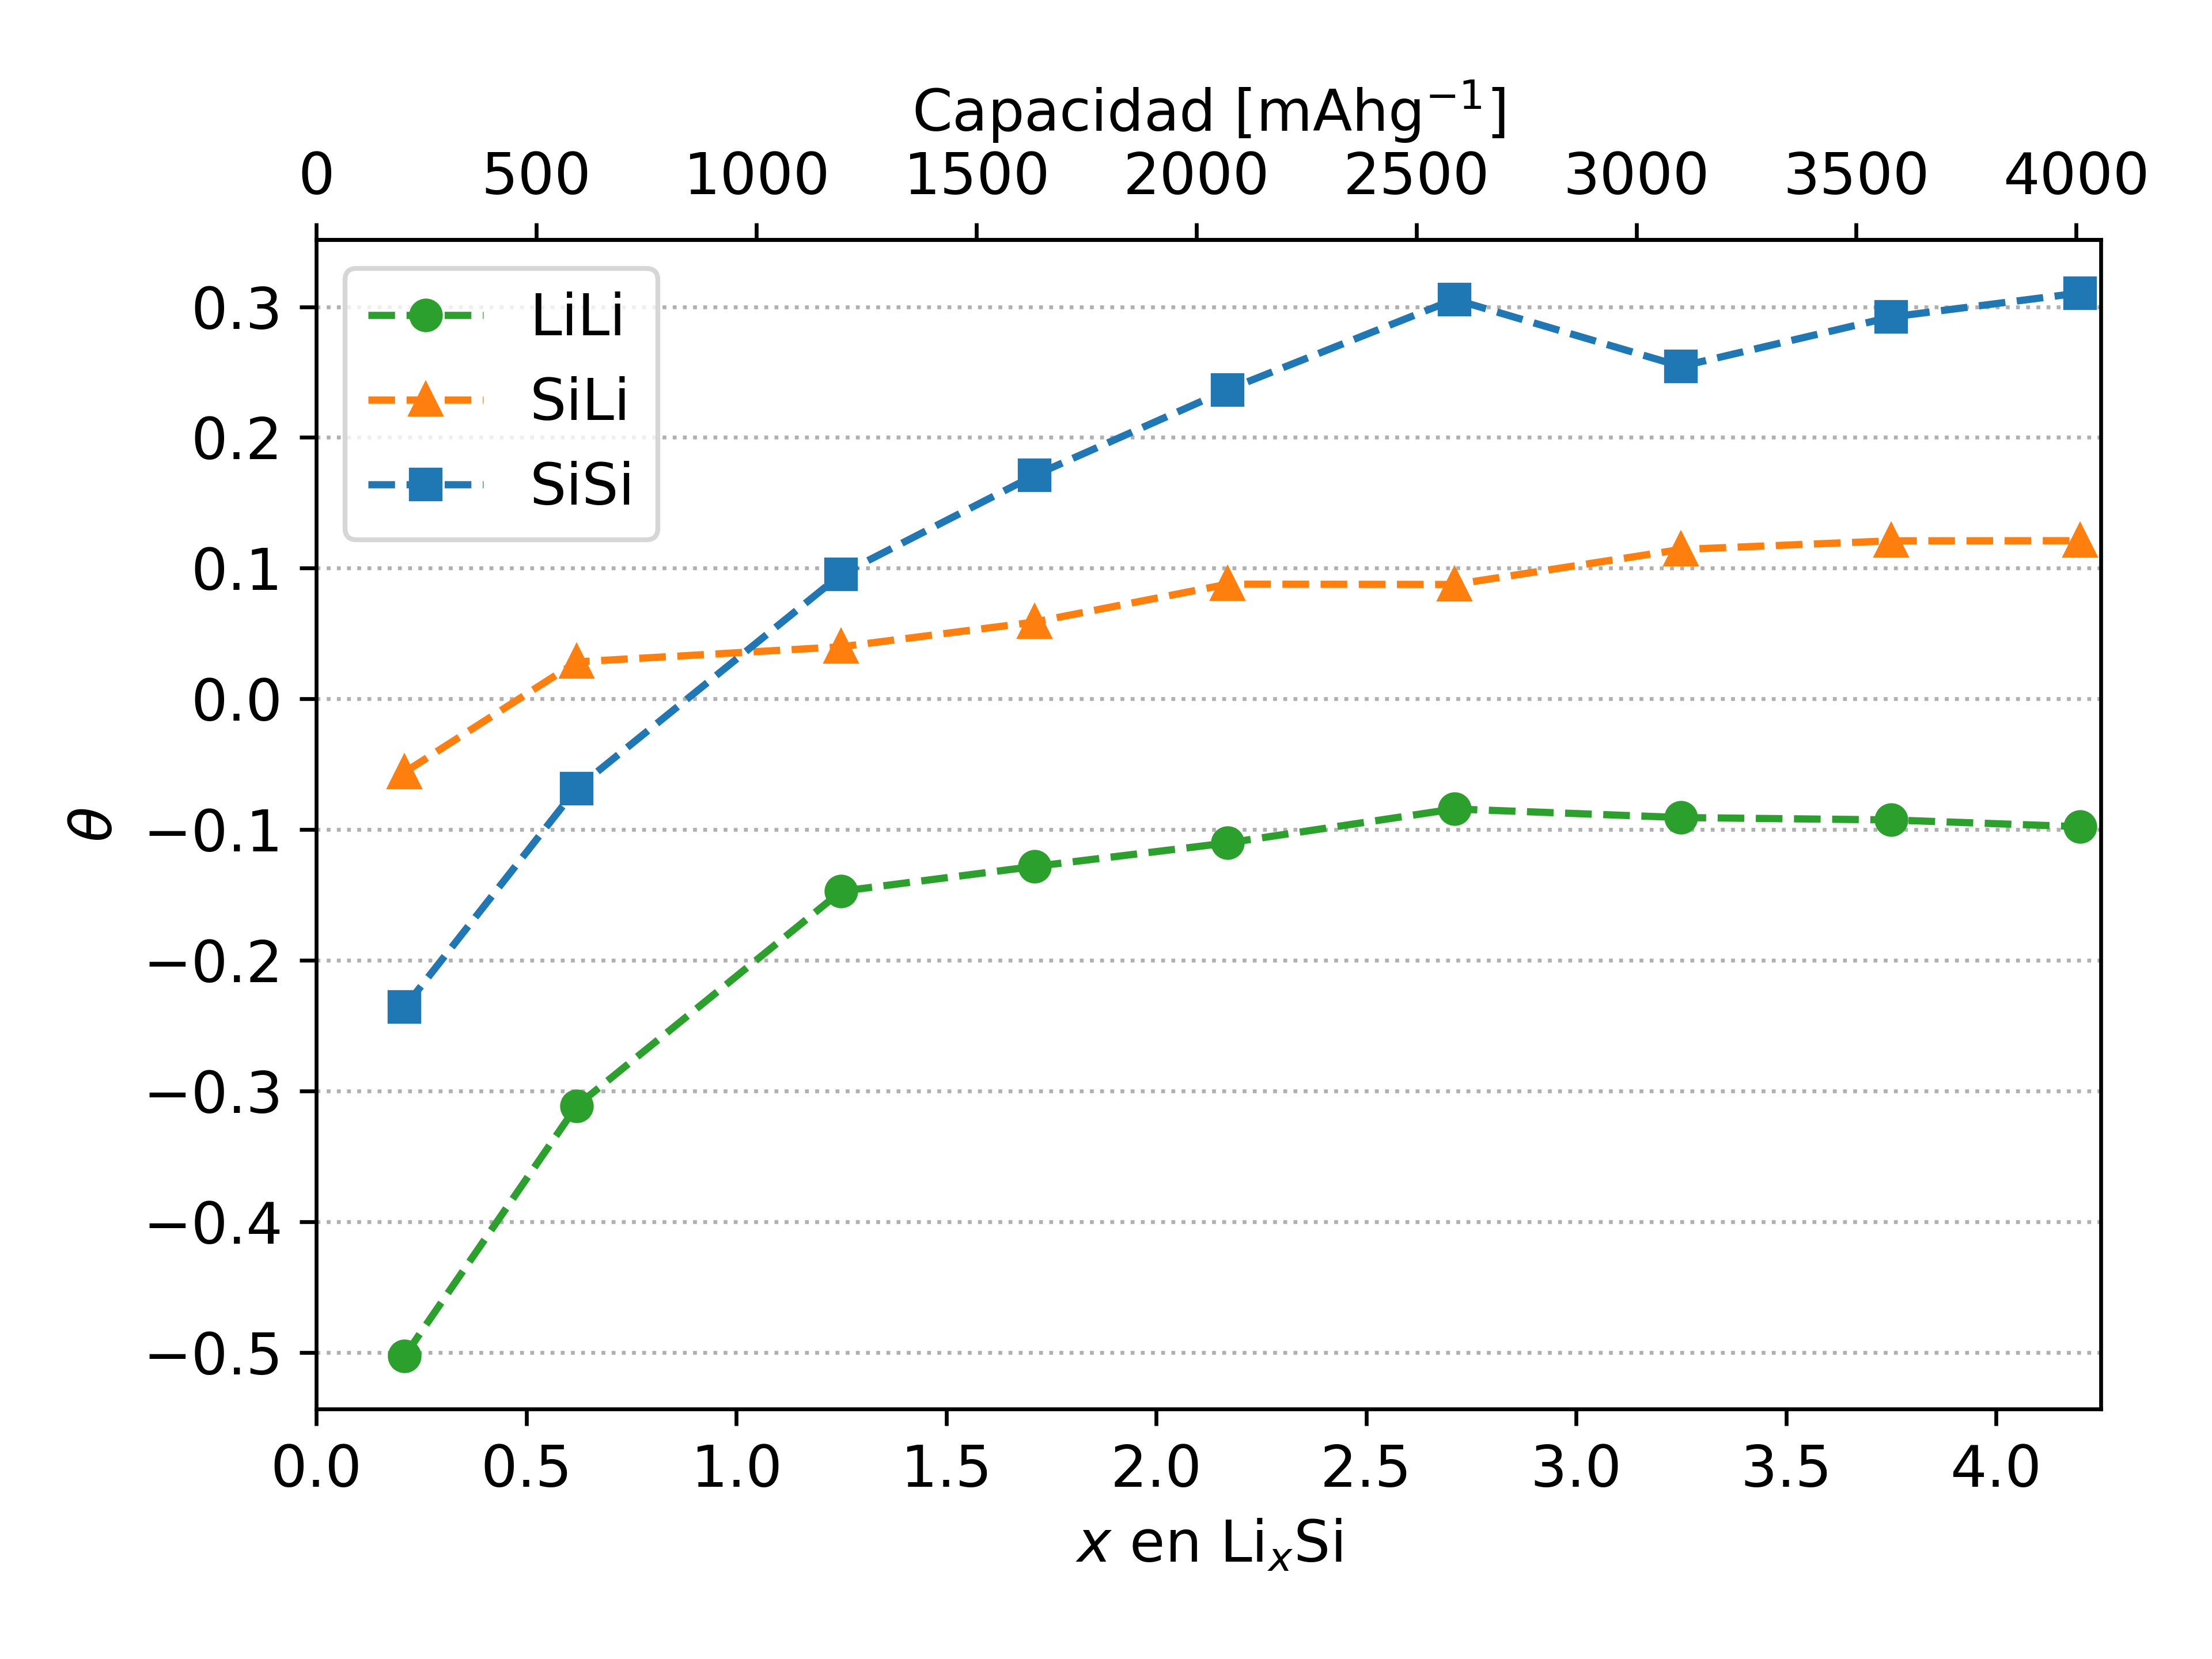
\includegraphics[width=0.7\textwidth]{Silicio/caracterizacion/resultados/sro/sro.png}
    \caption{Parámetros $\theta_{\text{Li}-\text{Li}}$, $\theta_{\text{Si}-\text{Li}}$ y $\theta_{\text{Si}-\text{Si}}$ 
    en función de la concentración de Li. El primer subíndice indica el tipo de
    átomo que se considera como central mientras que el segundo es el vecino. El
    radio de corte se eligió luego del primer pico de la RDF correspondiente.}
    \label{fig:sro}
\end{figure}

Como tendencia general, puede notarse que todos los valores de $\theta$ aumentan
cuando crece la cantidad de litio en el sistema, $x$, y que se estabiliza para 
valores grandes de $x$. Este comportamiento monótono y la disminución en la 
pendiente para concentraciones altas está correlacionado con el comportamiento
presentado en el análisis de los números de coordinación.

En el caso de $\theta_{\text{Si}-\text{Si}}$, éste alcanza un valor positivo aproximadamente 
constante para $x > 2.5$, mostrando una correlación fuerte con la presencia de 
cadenas lineales de Si, previamente discutidas y observadas en la Figura 
\ref{fig:amorfas}. Aunque la presencia de estas cadenas se puede inferir a partir
de los valores de los CN en $x$ altos, $\theta$ es más sensible al SRO, ya que
está normalizado por la concentración global. Esta propiedad de $\theta$ permite
un análisis más claro incluso si las cadenas están interactuando entre sí, como
es el caso para concentraciones bajas de litio.

$\theta_{\text{Si}-\text{Li}}$ presenta variaciones pequeñas y un valor positivo para todo 
$x > 0.5$, mostrando una acumulación constante de Li al rededor del Si, o, 
análogamente, una acumulación de Si alrededor del Li. Este comportamiento se le 
puede atribuir a la interacción atractiva fuerte en los pares Si-Li. En el caso de 
$\theta_{\text{Li}-\text{Li}}$, este parámetro es siempre negativo, lo que indica una 
interacción débil Li-Li y la correspondiente disminución de vecinos Li-Li. Por
último, el parámetro $\theta_{\text{Si}-\text{Si}}$ tiene un valor negativo para $x < 1.0$, 
sugiriendo que la presencia de concentraciones bajas de litio tiende a separar 
los átomos de silicio entre sí. Sin embargo, $\theta_{\text{Si}-\text{Si}}$ se vuelve positivo
para $x > 1.0$, implicando una acumulación de vecinos de Si sobre átomos de Si, 
relativo a la concentración global. Esto se debe a la formación de estructuras 
Si-Si. Para $x > 2.5$ puede observarse un valor constante de 
$\theta_{\text{Si}-\text{Si}} \approx 0.3$, revelando la formación de estructuras estables de 
Si-Si dadas por las cadenas previamente mencionadas.
